\documentclass[handout,a4paper,slidestop,xcolor=pst,blue]{beamer}

\usepackage{beamerthemesplit}
\usepackage[utf8]{inputenc}
\usepackage[spanish]{babel}
\usepackage{graphicx}
\usepackage{pstricks} % PSTricks package
\usepackage{setspace}
\usepackage{multirow}
\usepackage{listings}
\usepackage{pgfpages}
\usepackage{hyperref}
\usepackage{etoolbox}
\usepackage{epstopdf}

\makeatletter
\patchcmd{\beamer@sectionintoc}{\vskip1.5em}{\vskip0.5em}{}{}
\makeatother

\setbeamercovered{dynamic}
\setcounter{tocdepth}{2}
\setbeamercolor{frametitle}{fg=black,bg=white}
\setbeamercolor{section in toc shaded}{fg=black}
\setbeamercolor{section in toc}{fg=red}
\setbeamercolor{subsection in toc shaded}{fg=black}
\setbeamercolor{subsection in toc}{fg=red}
\setbeamerfont{section in toc}{size=\small}
\setbeamerfont{subsection in toc}{size=\small}
\setbeamertemplate{section in toc shaded}[default][99]
\setbeamertemplate{subsection in toc shaded}[default][99]

\AtBeginSection[]
{\begin{frame}[c]
  \frametitle{Índice}
	\tableofcontents[currentsection,
        sectionstyle=show/shaded,
        subsectionstyle=hide]
\end{frame}}

\AtBeginSubsection[]
{\begin{frame}[c]
	\frametitle{Índice}
	\tableofcontents[
  		currentsection,
  		sectionstyle=shaded/shaded,
  		currentsubsection,
  		subsectionstyle=show/shaded/hide
		]
\end{frame}}

\setbeamercolor{frametitle}{fg=black,bg=white}

\setbeamertemplate{frametitle}{
	\begin{centering}
		\insertframetitle
		\par
	\end{centering}
}

\usetheme[secheader]{Boadilla} 

\title[Modelo de Dominio]{Capa de Negocio - Modelo de Dominio}

\author[P. Sanchez]{\alert{Pablo Sánchez}}

\institute[IIE]{
		   Dpto. Ingeniería Informática y Electrónica \\
		   Universidad de Cantabria \\
		   Santander (Cantabria, España) \\
		   \texttt{p.sanchez@unican.es}
}

\date{}

\begin{document}

\begin{frame}[c]
	\titlepage
	\begin{columns}
		\column{0.50\linewidth}
			\centering
   		     
\includegraphics[width=.28\textwidth,keepaspectratio=true]{images/istr.eps}
		\column{0.50\linewidth}
			\centering
			
\includegraphics[width=.25\textwidth,keepaspectratio=true]{images/uc.eps}
	\end{columns}
\end{frame}

\begin{frame}[c]
	\frametitle{\alert{Advertencia}}
	\begin{center}
	Todo el material contenido en este documento no constituye en modo alguno una obra de referencia o apuntes oficiales mediante el cual se pueda preparar las pruebas evaluables necesarias para superar la asignatura. 
	\ \\ \ \\
	Este documento contiene exclusivamente una serie de diapositivas cuyo objetivo es servir de complemento visual a las actividades realizadas en el aula para la transmisión del contenido sobre el cual versarán las mencionadas pruebas evaluables.  
	\ \\ \ \\
	Dicho de forma más clara, \alert{estas diapositivas no son apuntes y su objetivo no es servir para que el alumno pueda preparar la asignatura de manera autónoma.}
	\end{center}
\end{frame}

\section{Introducción}

\begin{frame}[c]
    \frametitle{Objetivos del Tema}
    \begin{enumerate}[<+->]
         \item Comprender cuáles son las responsabilidades de la capa de negocio.
         \item Conocer los principales patrones de diseño relacionados con el desarrollo de una capa de negocio.
         \item Ser capaz de aplicar el patrón \emph{Domain Model}.
         \item Ser capaz de aplicar los principios de \emph{Domain-Driven Design}.
    \end{enumerate}
\end{frame}

\begin{frame}[c]
    \frametitle{Bibliografía}
    \begin{thebibliography}{1}

        \bibitem[Fowler, 2002]{Fowler2002x}
        Fowler, M. (2002).
        \newblock {\em {Patterns of Enterprise Application Architecture}}.
        \newblock Addison-Wesley.

        \bibitem[Evans, 2013]{Evans2003}
        Evans, E. J. (2003).
        \newblock {\em {Domain-Driven Design}}.
        \newblock Addison-Wesley.

        \bibitem[Esposito and Saltarello, 2014]{Esposito2014}
        Esposito, D. and Saltarello, A. (2014).
        \newblock {\em {Microsoft .NET - Architecting Applications for the
          Enterprise}}. 
        \newblock Microsoft Press. 2ª Edición.

    \end{thebibliography}
\end{frame}

\section{Capa de Negocio}

\begin{frame}
    \frametitle{Capa de Dominio}
    \only<1|handout:0>{
        \rput[lt](0,0){
            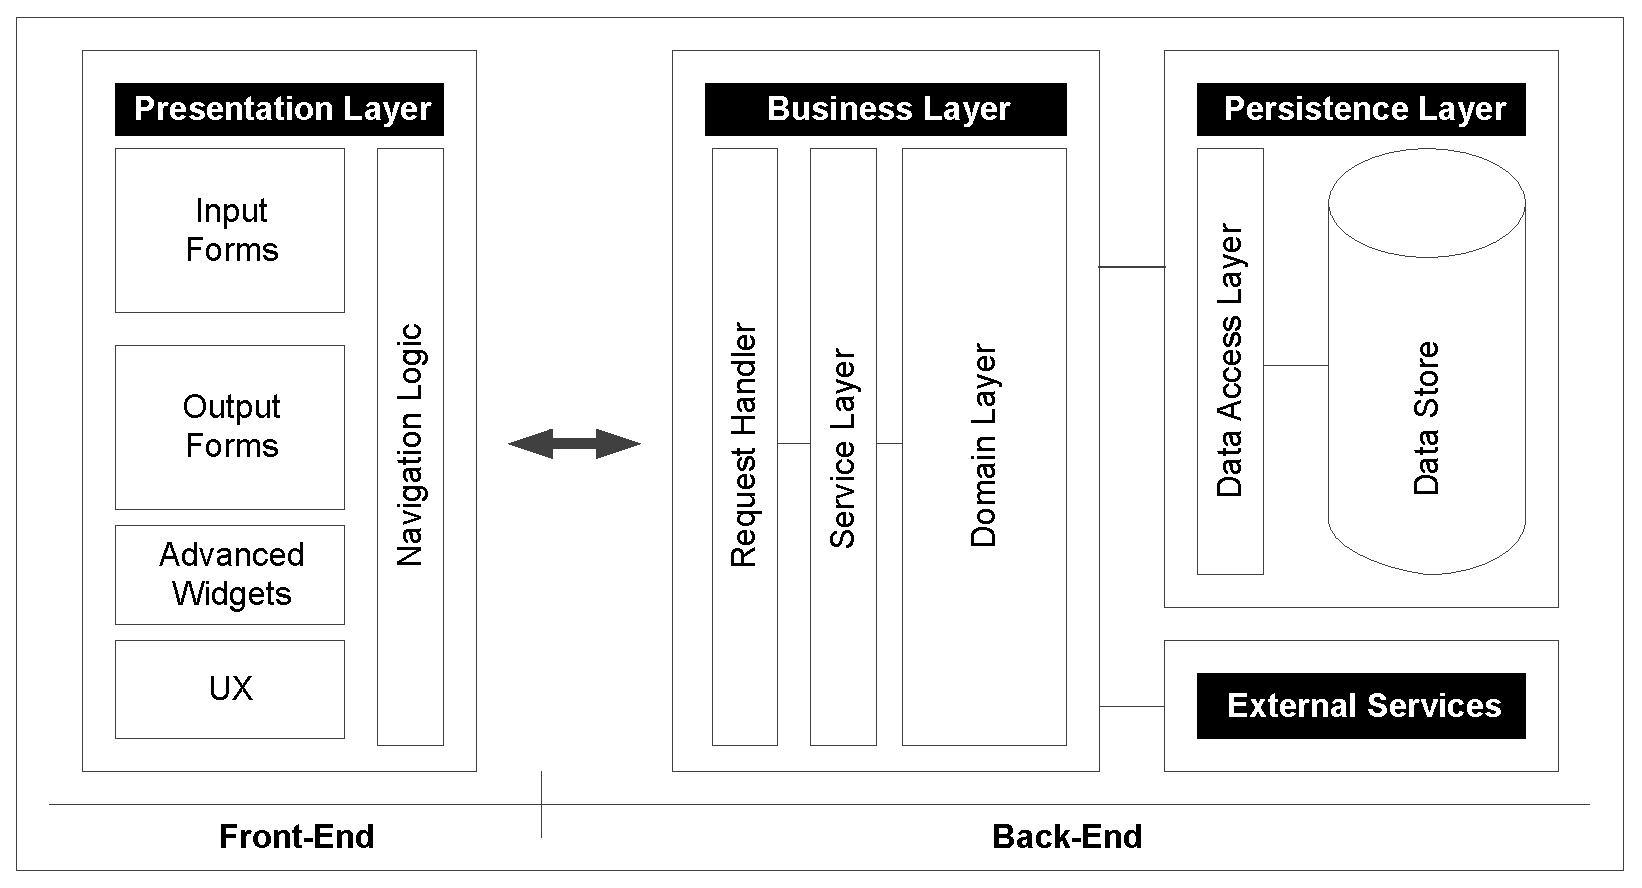
\includegraphics[width=\linewidth]{images/introduccion/enterpriseArchitectures00.eps}
        }
    }
    \only<2|handout:0>{
        \rput[lt](0,0){
            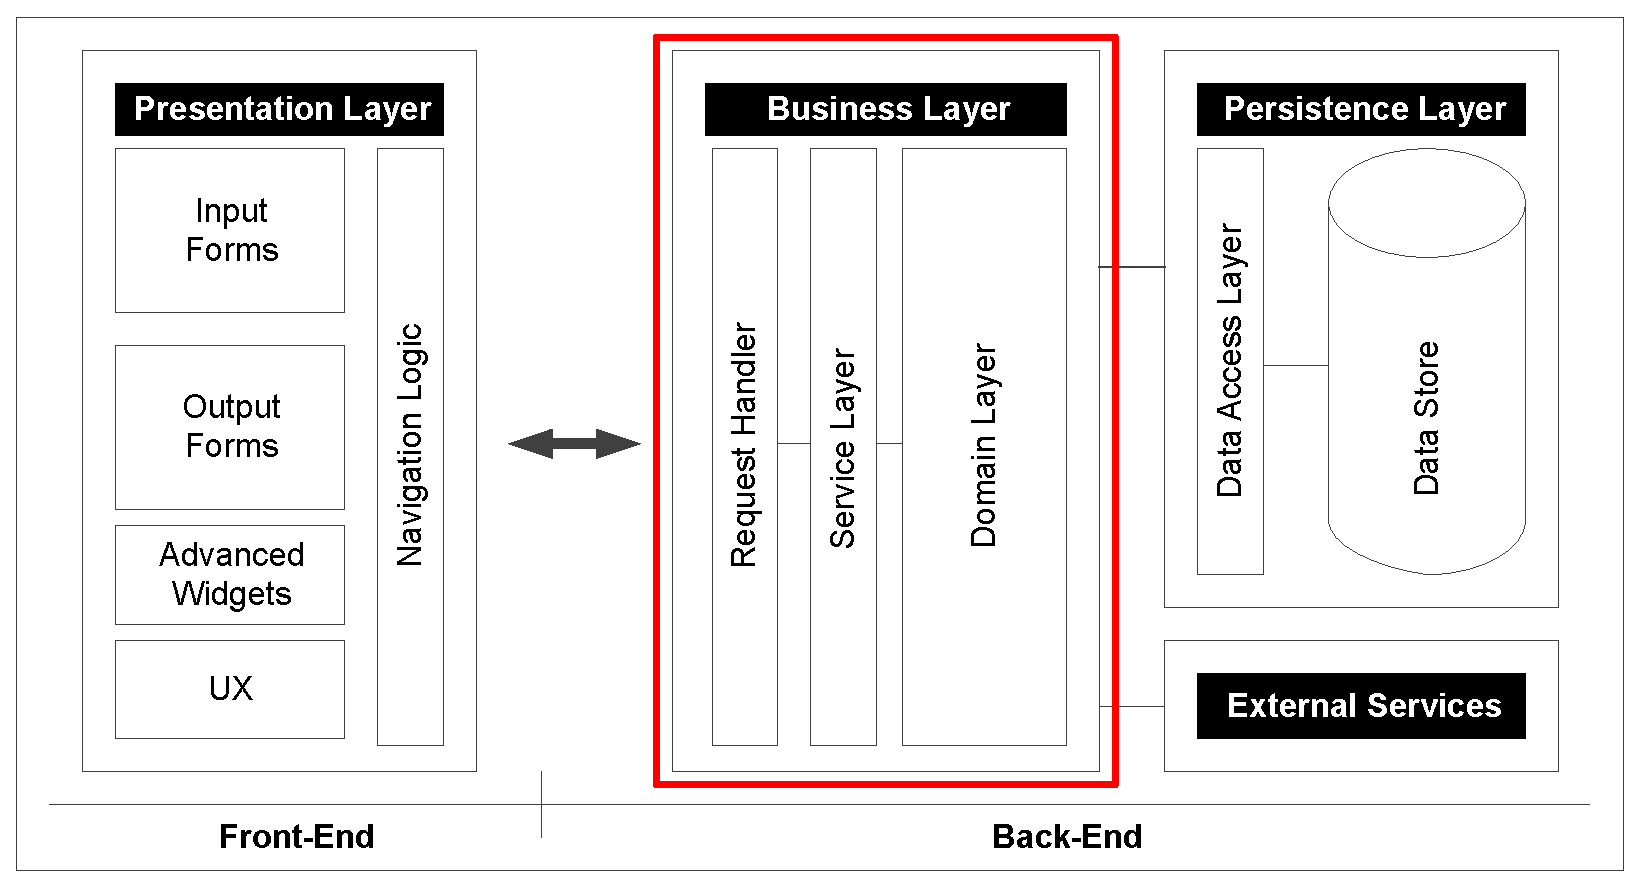
\includegraphics[width=\linewidth]{images/introduccion/enterpriseArchitectures01.eps}
        }
    }
    \only<3|handout:1>{
        \rput[lt](0,0){
            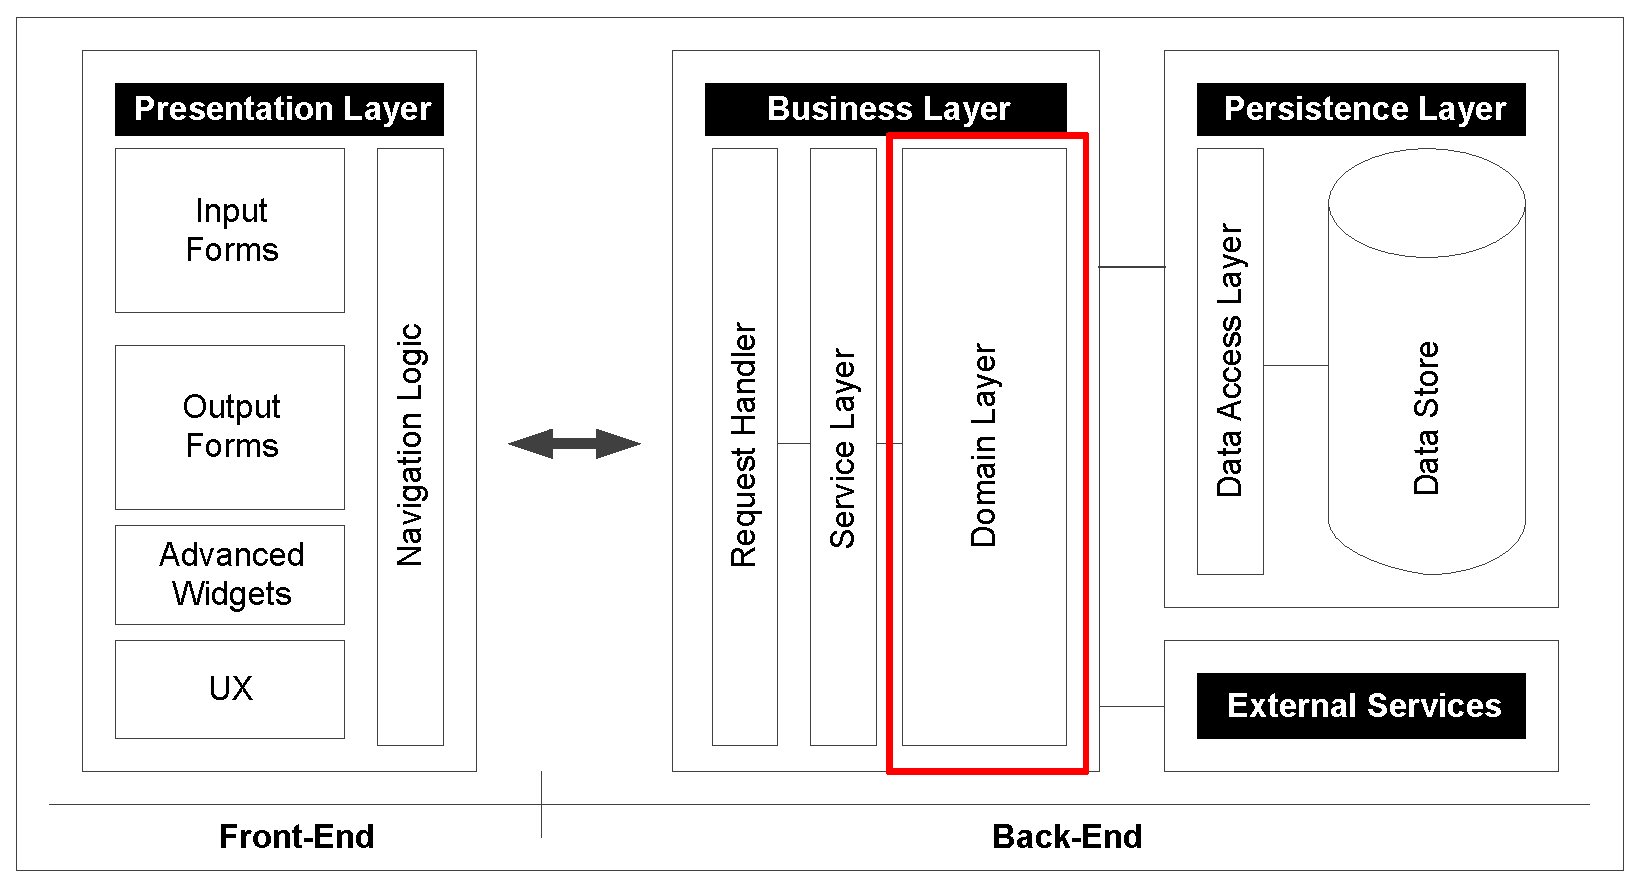
\includegraphics[width=\linewidth]{images/introduccion/enterpriseArchitectures02.eps}
        }
    }
\end{frame}

\begin{frame}[c]
	\frametitle{Responsabilidades de la Capa de Negocio}
	\begin{enumerate}[<+->]
        \item Atender las peticiones de los clientes.
        \item Asegurar el cumplimiento de \alert{reglas de negocio} existentes.
        \item Asegurar la \alert{transaccionalidad} de las operaciones de negocio.
        \item Validar las peticiones de los clientes.
        \item Recuperar y almacenar datos del almacén o almacenes persistentes.
        \item Facilitar la eficiencia del sistema.
        \item Controlar el acceso a los datos.
        \item Gestionar la comunicación con los servicios externos.
        \item Ejecutar operaciones (periódicas) del sistema.
        \item Gestionar de manera adecuada casos excepcionales.
        \item Ayudar a satisfacer los requisitos no funcionales.
	\end{enumerate}
\end{frame}

\section{Patrones para la Capa de Negocio}

\subsection{Problema Común}

\begin{frame}[c]
    \frametitle{Problema Común a los Patrones de la Capa de Negocio}
    \begin{block}{Problema Común}
        El problema común a los patrones de la capa de negocio es donde colocar la
        lógica de negocio de manera que se satisfagan las responsabilidades de la capa de negocio.
    \end{block}
    %% Poner ejemplo común
\end{frame}

\subsection{Table Module}

\begin{frame}[c]
    \frametitle{Table Module (obsoleto)}
    \begin{block}{Solución Table Module}
        Crear una clase que gestione la lógica de negocio de una tabla (o vista) completa. Conocido también como el \emph{Smart UI Antipattern}.
    \end{block}
    %% Poner ejemplo
    %% Crear ejemplo en GWT y subirlo a Git.
\end{frame}

\begin{frame}[c]
    \frametitle{Table Module (obsoleto)}
    \centering{\textbf{Ventajas}}
    \begin{enumerate}
        \item<2-> Facilidad de uso en lenguajes 4GL.
    \end{enumerate}
    \ \\ \ \\
    \uncover<3->{
        \centering{\textbf{Desventajas}}
        \begin{enumerate}
            \item<3-> Complica la manipulación de elementos individuales.
            \item<4-> Dificulta la gestión de datos residentes en varias tablas.
            \item<5-> Genera problemas de integración con otras aplicaciones.
            \item<6-> No utiliza orientación a objetos.
            \item<7-> Crea redundancias en la lógica de negocio.
            \item<8-> Dificulta la implementación de reglas de negocio complejas.
        \end{enumerate}
    }
\end{frame}

\subsection{Transaction Script}

\begin{frame}[c]
    \frametitle{Transaction Script (obsoleto)}
    \begin{block}{Solución Transaction Script}
        Crear un conjunto de funciones que respondan a los eventos que se puedan generar desde la interfaz de usuario, ejecutando para ello la lógica de negocio que sea necesaria.
    \end{block}
    %% Poner ejemplo
    %% Crear ejemplo y subirlo a Git.
\end{frame}

\begin{frame}[c]
    \frametitle{Transaction Script (obsoleto)}
    \centering{\textbf{Ventajas}}
    \begin{enumerate}
        \item<2-> Facilidad de implementación en aplicaciones sencillas.
    \end{enumerate}
    \ \\ \ \\
    \uncover<3->{
        \centering{\textbf{Desventajas}}
        \begin{enumerate}
            \item<4-> No utiliza orientación a objetos.
            \item<5-> Crea redundancias en la lógica de negocio.
            \item<6-> Dificulta la implementación de reglas de negocio complejas.
        \end{enumerate}
    }
\end{frame}

\subsection{Domain Model + Service Layer}

\begin{frame}[c]
    \frametitle{Domain Model}
    \begin{block}{Solución Domain Model}
        Modela el dominio del problema utilizando orientación a objetos y distribuye las reglas de negocio de manera adecuada entre las clases de dominio que corresponda.
    \end{block}
    %% Poner ejemplo
    %% Crear ejemplo y subirlo a Git.
\end{frame}

\begin{frame}[c]
    \frametitle{Domain Model}
    \centering{\textbf{Ventajas}}
    \begin{enumerate}
        \item<2-> Utiliza orientación a objetos.
        \item<3-> Reduce la redundancia en la lógica de negocio.
        \item<4-> Permite la utilización de patrones de diseño.
        \item<5-> Ofrece abstracciones más potentes para la implementación de reglas  de negocio complejas.
    \end{enumerate}
    \ \\ \ \\
    \uncover<7->{
        \centering{\textbf{Desventajas}}
        \begin{enumerate}
            \item<8-> Impedancia objeto-relacional u objeto-xxx.
            \item<9-> Mayor complejidad de diseño e implementación.
        \end{enumerate}
    }
\end{frame}

\begin{frame}[c]
    \frametitle{Service Layer}
    \begin{block}{Solución Domain Model}
        Aislar al modelo de dominio de otras capas y aplicaciones mediante la creación de una capa de servicio que:
        \begin{enumerate}
            \item<2-> Especifique las operaciones a las cuales es capaz de responder el modelo de dominio.
            \item<3-> Permita redirigir peticiones a las operaciones del modelo de dominio que correspondan, devolviendo la respuestas a los clientes de una manera adecuada.
            \item<4-> Permite encapsular la \emph{lógica de la aplicación} o \emph{workflow} (en caso de ser necesario).
        \end{enumerate}
    \end{block}
\end{frame}

\begin{frame}[c]
    \frametitle{Service Layer}
    \begin{block}{Lógica de la Dominio}
        La \emph{lógica de dominio} es el conjunto de procedimientos, restricciones y normas que rigen el funcionamiento de una determinada organización o dominio, y que son independientes de la existencia o no de una aplicación software.
    \end{block}
    \uncover<2->{
        \begin{block}{Lógica de la Aplicación}
            La \emph{lógica de la aplicación} es el conjunto de procedimientos, restricciones y normas que rigen el funcionamiento de una determinada aplicación. Es la encargada de gestionar elementos como transacciones, accesos a almacenes persistentes o seguridad.
        \end{block}
    }
\end{frame}

\begin{frame}[c]
    \frametitle{Service Layer}
    \begin{enumerate}
        \item<1-> Aisla al modelo de dominio de servicios concretos.
        \item<2-> Favorece la gestión de la lógica de la aplicación.
        \item<3-> Favorece la gestión de la concurrencia.
    \end{enumerate}
\end{frame}

\section{Domain-Driven Design}

\subsection{Introducción}

\begin{frame}[c]
    \frametitle{Domain-Driven Design}
     \begin{block}{Domain-Driven Design}
        \alert{\emph{Domain-Driven Design}} es una técnica de desarrollo sw donde todo el diseño de un producto sw gira en torno a un elemento central y fundamental que es el \emph{modelo de dominio}, el cual captura el dominio y la lógica de negocio de dicho producto sw.
     \end{block}
      %% Contar la historia de Monty Python
      %% Contar la historia del PCB
      %% Ventajas e Incovenientes: https://goo.gl/gPx5DE
      %% Add Page 8 documento de Evans.
\end{frame}

%%%\begin{frame}[c]
%%%    \frametitle{Domain-Driven Design}
%%%     \begin{block}{Ubiquitous Language}
%%%
%%%     \end{block}
%%%     %% Leer Capítulo 3 de Evans
%%%\end{frame}

\subsection{Entities}

\begin{frame}[c]
    \frametitle{Entities}
     \begin{block}{Entity}
        Una \emph{entity} es un objeto del dominio con una identidad y un ciclo de vida que debe ser reconocido y monitorizados.
     \end{block}
     \uncover<2->{
         \begin{block}{Características de un Identificador}
            %% Olvidarse del problema de las claves surrogadas de las bases de datos relacionales.
            \begin{enumerate}
                \item<3-> Únicos para cada objeto e inmutables.
                \item<4-> Pueden ser un único atributo o combinación de atributos.
                \item<5-> Si no se encuentra un identificador natural, puede ser generado por la aplicación.
                \item<6-> Si son generados, se esconden (normalmente) al usuario.
            \end{enumerate}
         \end{block}
     }
     %% Ejemplo de asiento en función numerada y no numerada.
     %% "Beyond identity issues, entities tend to fulfill their responsabilities
     %% by coordinating the operations of the objects they own"
\end{frame}

\subsection{Value Objects}

\begin{frame}[c]
    \frametitle{Value Objects}
    \begin{block}{Value Object}
        Elementos del dominio sin identidad definida, cuya existencia no es necesario monitorizar, y que simplemente representan valores de alguna propiedad de una entidad.
        %% Si me dan otro objeto, no tiene porque ser exactamente el mismo, me vale con que tenga
        %% sus mismas propiedades.
    \end{block}
    \uncover<2->{
         \begin{block}{Características de un \emph{Value Object}}
            %% Olvidarse del problema de las claves surrogadas de las bases de datos relacionales.
            \begin{enumerate}
                \item<3-> Dos instancias con los mismos valores se consideran idénticas, aunque tengan identidades distintas.
                \item<4-> Se recomienda hacer los \emph{value objects} inmutables.
            \end{enumerate}
        \end{block}
     }
\end{frame}

\subsection{Services}

\begin{frame}[c]
    \frametitle{Services}
    \begin{block}{Service}
        Un \emph{service} encapsula operaciones de dominio que no son responsabilidad natural de ninguna \emph{entity} o \emph{value object}.
    \end{block}
    \uncover<2->{
         \begin{block}{Características de un \emph{Service}}
            %% Declaración trimestal del IVA.
            \begin{enumerate}
                \item<3-> Forma parte del \emph{lenguaje universal} del dominio.
                \item<4-> Su interfaz está definida en base a otros elementos del modelo de dominio.
                \item<5-> Su operación u operaciones no tienen estado (\emph{stateless}).
            \end{enumerate}
        \end{block}
     }
\end{frame}

\subsection{Aggregates}

\begin{frame}[c]
    \frametitle{Aggregates}
    \begin{block}{Aggregate}
        Un \emph{aggregate} es un conjunto cohesionado de \emph{entities} y \emph{value objects} con una frontera clara con el resto del modelo de dominio y un conjunto de invariantes bien definidos que deben preservarse dentro de dicho conjunto.
    \end{block}
    \uncover<2->{
        \begin{block}{Aggregate Root}
            Dentro de un \emph{aggregate}, el \emph{aggregate root} es una \emph{entity} que controla el ciclo de vida del resto de los elementos del \emph{aggregate} y que contiene la información necesaria para encargarse de la preservación de los invariantes.
        \end{block}
    }
\end{frame}

\begin{frame}[c]
    \frametitle{Características de los \emph{Aggregates}}
    \begin{enumerate}[<+->]
        %% Alumno y expediente
        \item El \emph{aggregate root} debe tener identidad global.
        \item El resto de elementos del \emph{aggregate} sólo necesita tener identidad local.
        \item El \emph{aggregate root} es el encargado de preservar los invariantes.
        \item El tiempo de vida de un \emph{aggregate} debe ser uniforme a sus miembros.
        \item Los elementos externos al \emph{aggregate} sólo deben referenciar al \emph{aggregate root}.
        \item Los elementos internos de un \emph{aggregate} sólo pueden referenciar como elementos externos \emph{aggregate roots}.
        \item Los elementos internos de un \emph{aggregate} sólo deben utilizarse de manera transitoria fuera del \emph{aggregate}.
        \item Sólo los \emph{aggregate roots} pueden ser recuperados de persistencia.
        \item Si se elimina un \emph{aggregate root}, se debe eliminar todo el \emph{aggregate}.
    \end{enumerate}
\end{frame}

\subsection{Repositories}

\begin{frame}{c}
    \frametitle{Repositories}
    \begin{block}{Repository}
        Un \emph{repository} representa una clase que, a nivel conceptual, representa una colección con todas las instancias de una determinado elemento del dominio. El repositorio debe además proporcionar métodos para recuperar conjuntos de instancias concretos dentro de dicha colección, añadir nuevas instancias o eliminarlas.
    \end{block}
\end{frame}

\begin{frame}[c]
    \frametitle{Características de los \emph{Repositories}}
    \begin{enumerate}[<+->]
        %% Alumno y expediente
        \item Sólo existirán \emph{repositories} para los \emph{aggregates root}.
        \item Normalmente, existirá un \emph{repository} por cada \emph{aggregate root}.
        \item Cada \emph{repository} contendrá las operaciones CRUD básicas, más un método para recuperar todas las instancias de un elemento del dominio.
        \item Además, cada \emph{repository} contendrá otros métodos de búsqueda o cálculo siempre y cuando sean necesarios.
        %% Ojo con los repositorios, no son mágicos.
    \end{enumerate}
\end{frame}

\subsection{Otros elementos DDD}

\begin{frame}[c]
    \frametitle{Otros elementos DDD}
    \begin{enumerate}[<+->]
        \item Factories.
        \item Domain Events.
        \item Modules.
    \end{enumerate}
\end{frame}

\section{Sumario}

\begin{frame}[c]
    \frametitle{¿Qué Tengo que Saber de Todo Esto?}
    \begin{enumerate}[<+->]
        \item Comprender las responsabilidades de la capa de negocio.
        \item Conocer cómo funcionan \emph{Table Module} y \emph{Transaction Script}.
        \item Comprender por qué \emph{Table Module} y \emph{Transaction Script} se usan muy poco.
        \item Comprender cómo funciona \emph{Domain Model} y \emph{Service Layer}.
        \item Comprender los principios de \emph{Domain-Driven Design (DDD)}
        \item Ser capaz de crear modelos de dominio conforme a los principios \emph{DDD}.
    \end{enumerate}
\end{frame}


\end{document}
